\documentclass[letterpaper,10pt]{article}
\usepackage[utf8]{inputenc}
\usepackage{graphicx}
\usepackage{caption}
\usepackage{enumitem}
\usepackage[hidelinks]{hyperref}
\usepackage{amsmath}
\usepackage{amssymb}
\usepackage{adjustbox}
\usepackage{float} 
\usepackage{wrapfig}
\usepackage{xcolor} % Para definir colores
\usepackage{listings} % Para listados de código
\usepackage{array}
\usepackage{pgfplots}


\usepackage[margin=1in]{geometry} % Agrega esta línea para establecer los márgenes
% Configuración de colores
\pgfplotsset{compat=1.18}
\definecolor{commentcolor}{rgb}{0,0.6,0}
\definecolor{stringcolor}{rgb}{0.58,0,0.82}
\definecolor{keywordcolor}{rgb}{0,0,1}
\definecolor{backcolour}{rgb}{0.95,0.95,0.92}
\definecolor{grisclaro}{rgb}{0.9, 0.9, 0.9}
\definecolor{crtitle}{RGB}{112,48,160}
\definecolor{darkgreen}{RGB}{64,154,3}
\hypersetup{
    colorlinks=true,
    linkcolor=blue,
    urlcolor=blue    
}

% Configuración del estilo de los listados de código
\lstset{
    language=Go, % Define el lenguaje del código (Scala en este caso)
    basicstyle=\ttfamily\small, % Estilo de fuente básico
    commentstyle=\color{commentcolor}\ttfamily,
    stringstyle=\color{stringcolor}\ttfamily,
    keywordstyle=\color{keywordcolor}\bfseries\ttfamily,
    backgroundcolor=\color{grisclaro}, % Color de fondo
    showstringspaces=false, % No mostrar espacios en cadenas como caracteres especiales
    numbers=left, % Números de línea a la izquierda
    numberstyle=\tiny\color{gray}, % Estilo de los números de línea
    breaklines=true, % Romper líneas largas
    captionpos=b, % Posición del título ('b' para abajo)
    frame=single % Marco alrededor del código
}

\begin{document}
\begin{titlepage}
    \begin{center}
    
    
    
\includegraphics[scale=0.35]{Images/RojoTransparenteUV.png} \vspace{0.5cm}
    
    \textsc{\Large Proyecto de curso } \vspace{0.5cm} % Thesis type
    
    
    \rule{14cm}{0.05cm} \vspace{0.4cm} % Horizontal line
    
    
    \Large{\textbf{   Moderando el extremismo de opiniones en una red social  }}\vspace{0.4cm} % Thesis title
    
    \rule{14cm}{0.05cm} \vspace{1.5cm} % Horizontal line
     
    \large{\textit{realizado por:}} \\
    \Large{{\color{crtitle} 
    \textsuperscript{1}Juan Camilo Narvaez Tascón - 202140112, \\
    \textsuperscript{2}Julián Ernesto Puyo Mora - 202226905,\\
    \textsuperscript{3}Cristian David Pachecho Torres - 20222743,\\
    \textsuperscript{4}Juan Sebastián Molina Cuéllar - 202224491}
    }  %AUTHOR
    
    \vspace{2cm}
    
    \large \textit{
    Informe realizado para el curso de Análisis y Diseño de Algoritmos II,\\
    Profesor: Juan Francisco Díaz Frías - Profesor: Jesús Alexander Aranda\\
    Monitor: Mauricio Muñoz} 
    
    \vspace{0.3cm} % University requirement text
    
    \textit{de la}
    
    \vspace{0.4cm}
    
    Escuela de Ingeniería de Sistemas y Computación,\\ 
    Facultad de Ingeniería,\\ 
    Universidad del Valle
    
    \vspace{1.0cm} 
    {\color{crtitle} \small \textit{  
        \textsuperscript{1}juan.narvaez.tascon@correounivalle.edu.co, 
        \textsuperscript{2}julian.puyo@correounivalle.edu.co, 
        \textsuperscript{3}cristian.pacheco@correounivalle.edu.co,
        \textsuperscript{4}juan.sebastian.molina@correounivalle.edu.co
    }}\\
    \today
     
    
    \end{center}
    \end{titlepage}
\newpage

\tableofcontents
\newpage
\section{Introducción}
\label{sec:introduccion}
El presente informe tiene como objetivo abordar el problema de moderar el extremismo de opiniones en una red social, aplicando diferentes estrategias de diseño como fuerza bruta, algoritmos voraces y programación dinámica.

Se realizará una comparación entre estas estrategias basándose en su complejidad y optimalidad.

Para la implementación del proyecto, se ha seleccionado el lenguaje de programación \href{https://go.dev/}{Golang}. Esperamos que este informe sea de su agrado y cumpla con las expectativas del curso.
\section{Definición de estructuras y funciones útiles}
A continuación se presentan las funciones auxiliares y tipos de datos utilizados para implementar las soluciones al problema de moderar el extremismo de opiniones en la red social.
\subsection*{Tipos de datos}
A continuación, se muestran los tipos de datos definidos para representar la red social y los agentes en la misma.
\subsubsection*{Red Social}
\begin{equation}
  \mathcal{R} \mathcal{S} = < AG, R\_max >
\end{equation}\label{eq:red_social}
\begin{equation}
  AG = < a_1, a_2, \ldots, a_n >
  \label{eq:agentes}
\end{equation}
\begin{equation}
  R\_max \in \mathbb{N}
  \label{eq:recursos}
\end{equation}

Donde $AG$ es un conjunto de agentes y $R\_max$ es la cantidad máxima de recursos disponibles.

\begin{lstlisting}[caption={Definición de red social}, label={lst:r_s}]
type Network struct {
    Agents    []Agent
    Resources uint64
}
\end{lstlisting}
\subsubsection*{Agente}

\begin{lstlisting}[caption={Definición de agente}, label={lst:agente}]
type Agent struct {
    Opinion     int8
    Receptivity float64
}
\end{lstlisting}
Donde un agente $a_i$ es una pareja: $<{o_i}{^{\mathcal{R} \mathcal{S}}}, {r_i}{^{\mathcal{R} \mathcal{S}}}>$.
\newpage
\subsubsection*{Extremismo de una red $\mathcal{R}\mathcal{S}$}
\begin{equation}
  Ext(\mathcal{R}\mathcal{S}) = \frac{\sqrt{\sum_{i=0}^{n-1}{({o_i}{^{\mathcal{R} \mathcal{S}}})^2}}}{n}
  \label{eq:extremismo}
\end{equation}

\begin{lstlisting}[caption={Implementación del extremismo}, label={lst:ext}]
// extremism calculates the extremism of the network. It returns a float64 value.
func extremism(network *Network) float64 {
	var sumOpinions float64

	for _, agent := range network.Agents {
		sumOpinions += float64(agent.Opinion) * float64(agent.Opinion)
	}

	return math.Sqrt(sumOpinions) / float64(len(network.Agents))
}
\end{lstlisting}
\subsubsection*{Aplicar una estrategia de moderación $Mod(\mathcal{R}\mathcal{S},E)$}
\begin{equation}
  Mod(\mathcal{R}\mathcal{S}, E) = \mathcal{R}\mathcal{S}'
\end{equation}\label{eq:mod}
donde,
\begin{equation}
  o_i^{\mathcal{R}\mathcal{S}'} = 
  \begin{cases} 
        o_i^{\mathcal{R}\mathcal{S}'} & \text{si } e_i = 0 \\
        0        & \text{si } e_i = 1 
  \end{cases}
  \label{eq:mod_opinion}
\end{equation}

\begin{lstlisting}[caption={Implementación del Mod}, label={lst:mod}]
// moderation applies the strategy to the network. It returns the network after applying the strategy.
func moderation(network *Network, strategy []byte) *Network {
	networkPrime := Network{
		Agents:    make([]Agent, len(network.Agents)),
		Resources: network.Resources,
	}

	for i, strategyValue := range strategy {
		networkPrime.Agents[i].Opinion = network.Agents[i].Opinion - network.Agents[i].Opinion*int8(strategyValue)
	}

	return &networkPrime
}
\end{lstlisting}
\newpage
\subsubsection*{Esfuerzo}
El valor de esfuerzo a modelar la red $\mathcal{R}\mathcal{S}$.
\begin{equation}
  Esfuerzo(\mathcal{R}\mathcal{S}, E) = \sum_{i=0}^{n-1} \left\lceil  |o_i^{\mathcal{R}\mathcal{S}} - o_i^{\mathcal{R}\mathcal{S}'}| \times (1 - r_i^{\mathcal{R}\mathcal{S}}) \right\rceil
  \label{eq:esfuerzo}
\end{equation}

Donde $E$ (estrategia) es una secuencia que indica qué opinión de qué agente se modera por medio de $E$.
\begin{lstlisting}[caption={Implementación del esfuerzo}, label={lst:esfuerzo}]
  // effort calculates the effort of the network after applying the strategy. It returns a float64 value.
  func effort(network *Network, strategy []byte) float64 {
    n := len(network.Agents)
    networkPrime := moderation(network, strategy)
  
    var effortValue float64
    for i := 0; i < n; i++ {
      diff := float64(network.Agents[i].Opinion - networkPrime.Agents[i].Opinion)
      effortValue += math.Ceil(math.Abs(diff) * (1 - network.Agents[i].Receptivity))
    }
  
    return effortValue
  }
\end{lstlisting}
\section{Solución con Fuerza Bruta}
\label{sec:fuerza_bruta}

\subsection{Descripción del Algoritmo}
\label{subsec:descripcion_fuerza_bruta}
El enfoque de fuerza bruta para abordar el problema de moderar el extremismo se basa en generar todas las posibles estrategias de moderación \( E \) para una red social \( \mathcal{R}\mathcal{S} \) y seleccionar aquella estrategia que minimice el extremismo de la red social después de su aplicación, respetando la restricción de recursos \( R\_max \).

Formalmente, esto se expresa como:

\[
 AG \in \mathcal{R}\mathcal{S} \rightarrow \exists E = \langle e_0, e_1, \ldots, e_n \rangle \mid Esfuerzo(\mathcal{R}\mathcal{S}, E) \leqslant R\_max ~ \wedge ~ \min(Ext(Mod(\mathcal{R}\mathcal{S}, E)))
\]

Donde \( E \) es la estrategia de moderación aplicada a los agentes de la red social \( \mathcal{R}\mathcal{S} \), y la solución óptima es aquella que minimiza el extremismo \( Ext \) sin exceder los recursos disponibles "$\min(Ext(Mod(\mathcal{R}\mathcal{S}, E)))$".

\subsubsection*{Generación de Estrategias (StrategyGenerator)}
El primer paso es generar todas las posibles estrategias de moderación para una red social con \( n \) agentes. Para ello, se utiliza la función \( StrategyGenerator \) que genera todas las combinaciones posibles de estrategias de moderación.
\begin{lstlisting}[caption={Strategy Generator}, label={lst:strategy_generator}]
func StrategyGenerator(n int) [][]byte {
  total := 1 << n
  combinations := make([][]byte, total)
  
  for i := 0; i < total; i++ {
    combination := make([]byte, n)
    for j := 0; j < n; j++ {
      combination[n-j-1] = byte((i >> j) & 1)
    }
    combinations[i] = combination
  }

  return combinations
}
\end{lstlisting}
\textit{Esta función genera todas las posibles estrategias de moderación para una red social con \( n \) agentes. Cada estrategia es representada por una secuencia de \( n \) bits, donde el bit \( i \) indica si el agente \( i \) es moderado o no.
}
\\

\textbf{Explicación del código:}
\begin{itemize}
  \item Se recibe como parámetro \(n\), el número de agentes, y se calcula el total de combinaciones posibles (\(2^n\)).
  \item Se crea un arreglo \textit{combinations} para almacenar todas las combinaciones posibles.
  \item Un ciclo \textit{for} itera sobre cada combinación posible. Dentro del ciclo:
  \begin{itemize}
    \item Se crea un arreglo \textit{combination} que representa una combinación específica de \(n\) bits.
    \item Otro ciclo \textit{for} asigna el valor de cada bit en la combinación utilizando operaciones de desplazamiento de bits.
    \item La combinación generada se guarda en el arreglo \textit{combinations}.
  \end{itemize}
  \item Al final, se retorna el arreglo que contiene todas las combinaciones generadas.
\end{itemize}
\subsubsection*{Algoritmo de Moderación (ModexFB)}
\begin{lstlisting}[caption={Algoritmo de Fuerza Bruta}, label={lst:modexfb}]
func ModexFB(network *Network) (bestStrategy []byte, bestEffort float64, minExtremism float64, err error) {
  numAgents := len(network.Agents)
  
  if numAgents > 25 {
    return nil, 0, 0, errors.New("In ModexFB the number of agents must be less than or equal to 25")
  }

  var possibleStrategies [][]byte = strategyGenerator(numAgents)
  minExtremism = math.Inf(1)
  bestEffort = math.Inf(1)
  
  for _, strategy := range possibleStrategies {
    effortValue, networkPrime := effort(network, strategy)
    if effortValue <= float64(network.Resources) {
      extremismValue := extremism(networkPrime)
      if extremismValue < minExtremism {
        minExtremism = extremismValue
        bestEffort = effortValue
        bestStrategy = strategy
      }
    }
  }
  return bestStrategy, bestEffort, minExtremism, nil
}
\end{lstlisting}
\textit{La función \textit{ModexFB} recibe por parametro la red de agentes y retorna la mejor estrategia , el esfuerzo asociado , el extremismo mínimo.}
\\
\\
\\
\textbf{Explicación del código:}
\begin{itemize}
  \item Se inicializa el número de agentes (\textit{numAgents}) y, si es mayor a 25, se retorna un error.
  \item Se generan todas las estrategias posibles con \textit{strategyGenerator} y se inicializan \textit{minExtremism} y \textit{bestEffort} con valores infinitos.
  \item Un ciclo \textit{for} recorre cada estrategia posible, calculando el esfuerzo (\textit{effortValue}) y el extremismo (\textit{extremismValue}) resultante.
  \item Si el esfuerzo es menor o igual a los recursos disponibles y el extremismo es menor al mínimo registrado, se actualizan las variables \textit{bestStrategy}, \textit{bestEffort}, y \textit{minExtremism}.
  \item Al final, se retorna la mejor estrategia encontrada junto con el esfuerzo y el extremismo mínimo.
\end{itemize}


Este algoritmo de fuerza bruta genera todas las posibles estrategias de moderación y selecciona la mejor según dos criterios: esfuerzo mínimo y extremismo mínimo, siempre que el esfuerzo no exceda los recursos de la red.


\subsection{Complejidad}
\label{subsec:complejidad_fuerza_bruta}
Para analizar la complejidad del algoritmo debemos de considerar los dos ciclos \textit{for} que ocurren dentro del código, el primer ciclo (linea 11) hace un recorrido sobre todas las posibles combinaciones de agentes que existen (linea 8 \textit{total = 1 $<<$ numAgents}), y el segundo ciclo (linea 13) hace un recorrido por el total de agentes (linea 2 \textit{numAgents:= len(network.Agents)}).

\textbf{Entonces tenemos que:}
\begin{itemize}
  \item El primer ciclo tiene una complejidad de \(O(2^n)\), debido a que $e_i$ puede tomar dos valores ($0$ o $1$) donde \(n\) es el número de agentes en la red social.
  \item El segundo ciclo tiene una complejidad de \(O(n)\), donde \(n\) es el número de agentes en la red social.
\end{itemize}
Debido a que los demás cálculos internos realizados son de complejidad \(O(1)\), la complejidad total del algoritmo es \(O(2^n \cdot n)\).
\subsection{Corrección}
\label{subsec:correccion_fuerza_bruta}
Sea $RS$ una red social con $n$ agentes $AG = \{a_1, a_2, \dots, a_n\}$.

Definimos una estrategia de moderación como un vector:

\[
E = \langle e_1, e_2, \dots, e_n \rangle
\]

donde:
\begin{itemize}
  \item $e_i \in \{0, 1\}$ para $1 \leq i \leq n$.
  \begin{itemize}
    \item $e_i = 1$: el agente $a_i$ es moderado.
    \item $e_i = 0$: el agente $a_i$ no es moderado.
  \end{itemize}
\end{itemize}

El conjunto de todas las estrategias posibles es:

\[
\mathcal{E} = \{\langle e_1, e_2, \dots, e_n \rangle \mid e_i \in \{0, 1\} \, \forall i\}
\]

\subsubsection*{Número total de estrategias posibles}

Cada agente tiene 2 opciones (ser moderado o no), y hay $n$ agentes. Por lo tanto, el número total de estrategias posibles es:

\[
|\mathcal{E}| = 2^n
\]

\subsubsection*{Análisis de la función \textit{strategyGenerator(n)} (\ref{lst:strategy_generator})}

Descripción de la función:

La función \textit{strategyGenerator(n)} (\ref{lst:strategy_generator}) genera todas las posibles combinaciones de estrategias para $n$ agentes. Lo hace de la siguiente manera:

\begin{itemize}
    \item Calcula el total de combinaciones posibles: $total = 2^n$.
    \item Itera desde $i = 0$ hasta $i = 2^n - 1$.
    \item Para cada $i$, genera una combinación binaria de longitud $n$, donde cada bit representa $e_j$ para el agente $a_j$.
\end{itemize}

\textbf{Demostración de que genera todas las estrategias}
\\

\textbf{Cobertura completa}: El rango de $i$ desde $0$ hasta $2^n - 1$ asegura que se cubren todas las posibles combinaciones binarias de longitud $n$.

\textbf{Correspondencia uno a uno}: Cada entero $i$ en este rango tiene una representación binaria única de $n$ bits. Esta representación binaria se asigna directamente a una estrategia $E = \langle e_1, e_2, \dots, e_n \rangle$, donde $e_j$ es el bit $j$ de $i$.

\textbf{Conclusión}: La función \textit{strategyGenerator(n)} (\ref{lst:strategy_generator}) genera exactamente todas las $2^n$ estrategias posibles en $E$, sin omitir ni repetir ninguna.

\subsubsection*{Funcionamiento del algoritmo \textit{ModexFB}}

\textbf{Paso a paso del algoritmo}
\\

\textbf{Generación de estrategias}:
\begin{itemize}
    \item Llama a \textit{strategyGenerator(n)} (\ref{lst:strategy_generator}) para obtener el conjunto completo de estrategias posibles $E$.
\end{itemize}

\textbf{Inicialización de variables}:
\begin{itemize}
    \item Establece \textit{minExtremism} y \textit{bestEffort} con valores iniciales infinitos. Estas variables almacenarán el extremismo mínimo encontrado y el esfuerzo correspondiente.
\end{itemize}

\textbf{Evaluación de cada estrategia}:
\begin{itemize}
    \item Recorre cada estrategia $E \in \mathcal{E}$.
    \item Para cada estrategia:
    \begin{itemize}
        \item Calcula el esfuerzo total requerido para aplicar $E$ usando la función \textit{effort(network, strategy)} (\ref{lst:esfuerzo}).
        \item Si el esfuerzo total es menor o igual a los recursos disponibles $R_{max}$, procede a calcular el extremismo resultante.
        \item Utiliza la función \textit{extremism(networkPrime)}(\ref{lst:ext}) para obtener el extremismo de la red después de aplicar $E$.
        \item Si el extremismo resultante es menor que \textit{minExtremism}, actualiza:
        \begin{itemize}
            \item \textit{minExtremism} con el nuevo valor de extremismo.
            \item \textit{bestEffort} con el esfuerzo total de la estrategia actual.
            \item \textit{bestStrategy} con la estrategia actual $E$.
        \end{itemize}
    \end{itemize}
\end{itemize}

\textbf{Resultado final}:
\begin{itemize}
    \item Después de recorrer todas las estrategias en $E$, el algoritmo devuelve:
    \begin{itemize}
        \item \textit{bestStrategy}: la estrategia que minimiza el extremismo sin exceder $R_{max}$.
        \item \textit{bestEffort}: el esfuerzo total de \textit{bestStrategy}.
        \item \textit{minExtremism}: el extremismo mínimo logrado.
    \end{itemize}
\end{itemize}

Dado que el algoritmo recorre todas las estrategias en $\mathcal{E}$ sin excepción, y para cada una realiza las evaluaciones necesarias, asegura que ninguna estrategia posible es omitida. Por lo tanto, el algoritmo considera todas las posibles combinaciones de estrategias $E$.

\subsubsection*{ModexFB mejorado}

Debido a que el ciclo realizado en la función \textit{ModexFB} (\ref{lst:modexfb}) recorre todas las estrategias posibles, además de en la línea 18 llamar a \textit{strategyGenerator} (\ref{lst:strategy_generator}) pero para evitar la exploración de estrategias inecesarias y además en el mismo recorrido calcular el esfuerzo y el extremismo de la red, se puede mejorar el algoritmo de la siguiente manera:
\begin{lstlisting}[caption={ModexFB mejorado}, label={lst:modexfb_mejorado}]
func ModexFB(network *Network) (bestStrategy []byte, bestEffort float64, minExtremism float64, err error) {
	numAgents := len(network.Agents)

	if numAgents > 25 {
		return nil, 0, 0, errors.New("In ModexFB the number of agents must be less than or equal to 25")
	}

	total := 1 << numAgents
	minExtremism = math.Inf(1)

	for i := 0; i < total; i++ {
		strategy := make([]byte, numAgents)
		for j := 0; j < numAgents; j++ {
			strategy[numAgents-j-1] = byte((i >> j) & 1)
		}
		effortValue, networkPrime := effort(network, strategy)
		if effortValue <= float64(network.Resources) {
			extremismValue := extremism(networkPrime)
			if extremismValue < minExtremism {
				minExtremism = extremismValue
				bestEffort = effortValue
				bestStrategy = strategy
			}
		}
	}

	return bestStrategy, bestEffort, minExtremism, nil
}
\end{lstlisting}
\section{Solución con Algoritmo Voraz}
\label{sec:algoritmo_voraz}
"Describen correctamente un algoritmo voraz para resolver el problema, calcula correctamente su complejidad y la justifica, y analiza acertadamente si el algoritmo da siempre la respuesta correcta y lo justifica. El algoritmo quedó clasificado en el grupo de los mejores voraces del curso."

Para la realización de este algoritmo, se consideró la relación que hay entre el $extremismoParcial$ $(O_i\mathcal{R} \mathcal{S})^2$ y el $esfuerzoParcial = \left\lceil  |o_i^{\mathcal{R}\mathcal{S}} - o_i^{\mathcal{R}\mathcal{S}'}| \times (1 - r_i^{\mathcal{R}\mathcal{S}}) \right\rceil$ para cada agente $a_i$ en la red social $\mathcal{R}\mathcal{S}$.

Sea:
\[
  esfuerzoParcial = \left\lceil  |o_n^{\mathcal{R}\mathcal{S}} - o_n^{\mathcal{R}\mathcal{S}'}| \times (1 - r_n^{\mathcal{R}\mathcal{S}}) \right\rceil
\]

De tal forma que para un agente $a_i$ en la red social $\mathcal{R}\mathcal{S}$, se moderará si se cumple:
\begin{equation}
  \frac{(O_i\mathcal{R} \mathcal{S})^2}{\left\lceil  |o_i^{\mathcal{R}\mathcal{S}} - o_i^{\mathcal{R}\mathcal{S}'}| \times (1 - r_i^{\mathcal{R}\mathcal{S}}) \right\rceil} \geqslant  \frac{(O_{i-1} \mathcal{R} \mathcal{S})^2}{\left\lceil  |o_{i-1}^{\mathcal{R}\mathcal{S}} - o_{i-1}^{\mathcal{R}\mathcal{S}'}| \times (1 - r_{i-1}^{\mathcal{R}\mathcal{S}}) \right\rceil}
  \label{eq:voraz}
\end{equation}
\begin{equation}
  \eqref{eq:voraz} | \sum_{i=1}^{l}esfuerzoParcial + esfuerzoParcial_i \leqslant Recursos
  \label{eq:voraz2}
\end{equation}
\subsection{Descripción del Algoritmo}
\label{subsec:descripcion_algoritmo_voraz}
Teniendo en cuenta lo explicado anteriormente se realizó el siguiente algoritmo:
\begin{lstlisting}[caption={Algoritmo Voraz}, label={lst:ModexV}]
func ModexV(network *Network) ([]byte, float64, float64, error) {
  if network == nil || len(network.Agents) == 0 {
    return nil, 0, 0, errors.New("network is nil or has no agents")
  }

  // Generate the greedy strategy.
  resources := network.Resources
  strategy := make([]byte, len(network.Agents))
  totalEffort := 0.0

  rankedAgents := rankAgents(network)

  for _, agentInfo := range rankedAgents {
    if uint64(totalEffort+agentInfo.Effort) <= resources {
      // Moderate the agent.
      strategy[agentInfo.Index] = 1
      totalEffort += agentInfo.Effort
    } else {
      // Do not moderate the agent.
      strategy[agentInfo.Index] = 0
    }
  }

  // Calculate the total effort and the moderated network.
  totalEffort, moderatedNetwork := effort(network, strategy)

  // Check if the total effort exceeds the available resources.
  if uint64(totalEffort) > network.Resources {
    return nil, 0, 0, errors.New("insufficient resources to apply the strategy")
  }

  // Calculate the new extremism after applying the strategy.
  newExtremism := extremism(moderatedNetwork)

  return strategy, totalEffort, newExtremism, nil
}
\end{lstlisting}
\textbf{Explicación del código:}
\begin{itemize}
  \item Primero, el algoritmo verifica si la red es nula o no tiene agentes. Si es así, retorna un error.
  \item Se inicializa la cantidad de recursos disponibles y se crea un arreglo \textit{strategy} para almacenar la estrategia de moderación, que contiene un 1 si el agente es moderado y un 0 si no lo es.
  \item Los agentes son ordenados de manera voraz usando una función \textit{rankAgents}, que los clasifica y los ordena en función de \eqref{eq:voraz2}.
  \item Un ciclo recorre la lista de agentes ordenados. Para cada agente:
  \begin{itemize}
    \item Si el esfuerzo acumulado más el esfuerzo del agente no excede los recursos disponibles, se modera al agente (se asigna 1 en \textit{strategy}).
    \item Si no hay suficientes recursos, el agente no es moderado (se asigna 0 en \textit{strategy}).
  \end{itemize}
  \item Una vez definida la estrategia, se calcula el esfuerzo total y se genera una versión moderada de la red con la función \textit{effort}.
  \item Si el esfuerzo total excede los recursos disponibles, se retorna un error.
  \item Finalmente, se calcula el extremismo resultante de la red moderada utilizando la función \textit{extremism} y se retorna la estrategia, el esfuerzo total y el nuevo extremismo.
\end{itemize}
\subsection{Análisis del Algoritmo}
\label{subsec:analisis_algoritmo_voraz}
Como podemos apreciar el algoritmo aplica la eurísitca mensionada en \eqref{eq:voraz} y \eqref{eq:voraz2} para moderar los agentes de la red social $\mathcal{R}\mathcal{S}$, de tal forma que se minimiza el extremismo de la red social sin exceder los recursos disponibles.

Pero ello tiene un problema, si la red social, no está ordenada en función de \eqref{eq:voraz2}, la eurística perderá precisión para el caso en que la red tenga los mejores casos de moderación al final de la lista de agentes.

Por ello se implementó la función \textit{rankAgents} que ordena los agentes en función de \eqref{eq:voraz2} de la siguiente manera:
\begin{lstlisting}[caption={Rank Agents}, label={lst:rank_agents}]
func rankAgents(network *Network) []AgentRatio {
  agentRatios := make([]AgentRatio, len(network.Agents))

  for i, agent := range network.Agents {
    extremism := float64(partialExtremism(agent))
    effort := partialEffort(agent)
    var ratio float64
    if effort == 0 {
      ratio = math.Inf(1) // Assign infinite ratio to agents with zero effort.
    } else {
      ratio = extremism / effort
    }

    agentRatios[i] = AgentRatio{
      Index:   i,
      Ratio:   ratio,
      Effort:  effort,
      Benefit: extremism,
    }
  }

  // Sort agents by descending ratio.
  sort.Slice(agentRatios, func(i, j int) bool {
    return agentRatios[i].Ratio > agentRatios[j].Ratio
  })

  return agentRatios
}
\end{lstlisting}
\textbf{Explicación del código:}
\begin{itemize}
  \item Se inicializa un arreglo \textit{agentRatios} de tamaño igual al número de agentes en la red.
  \item El ciclo \textit{for} recorre todos los agentes de la red. Para cada agente:
  \begin{itemize}
    \item Se calcula el extremismo parcial del agente (\textit{partialExtremism}) y el esfuerzo necesario para moderarlo (\textit{partialEffort}).
    \item Se determina la relación (\textit{ratio}) entre el extremismo y el esfuerzo. Si el esfuerzo es cero, se asigna una relación infinita (\textit{math.Inf(1)}), ya que moderar a este agente no requiere esfuerzo.
    \item La relación calculada, junto con el índice del agente, el esfuerzo y el extremismo, se almacena en el arreglo \textit{agentRatios}.
  \end{itemize}
  \item Una vez que se ha calculado la relación para todos los agentes, se ordenan por su relación de extremismo sobre esfuerzo en orden descendente usando la función \textit{sort.Slice}.
  \item El algoritmo retorna el arreglo \textit{agentRatios}, que ahora contiene a los agentes clasificados en función de la mayor relación $\frac{extremismoParcial}{esfuerzoParcial}$.
\end{itemize}
\textbf{¿Garantiza solución óptima?}

Como vimos anteriormente el algoritmo selecciona a los agentes en función de \eqref{eq:voraz2}, por lo que se garantiza que se seleccionan los agentes que minimizan el extremismo de la red social sin exceder los recursos disponibles. Más adelante podría no haber suficientes recursos para moderar otro agente que, en combinación con otros, habría resultado en un menor extremismo global si se hubieran elegido de manera diferente.

Debido a que no se evalúa las combinaciones posibles de agentes y recursos, sino que elige en cada paso lo que pareciera mejor en ese instante (euristica \eqref{eq:voraz2}), el algoritmo no garantiza la solución óptima global.

\subsection{Complejidad}
\label{subsec:complejidad_algoritmo_voraz}
Para determinar la complejidad del algoritmo voraz, se considera tres partes. La primera, donde la función \textit{rankAgents} (\ref{lst:rank_agents}), que recorre n agentes en un solo ciclo para determinar el ratio, dando su complejidad de ejecución de \(O(n)\). La segunda, esta dado por la función \textit{sort.Slice}, una función del paquetede sort de Go, cuya complejidad, según la documentación es \(O(log(n))\). Y la tercera parte, la aplicación de la decisión local del algoritmo voraz, la cual determina si incluir o no un determinado agente, en un recorrido para los n agentes, lo cual, nuevamente, representa una complejidad de \(O(n)\). Por lo tanto, la complejidad total del algoritmo voraz, considerando todas las partes, deviene a \(O(2n + log(n))\) .
\subsection{Corrección}
\label{subsec:correccion_algoritmo_voraz}
El algoritmo voraz propuesto \ref{lst:ModexV} no garantiza solución óptima global, como se mensionó anteriormente. 

Supongamos que:
\[
  \forall \mathcal{R}\mathcal{S}, \forall R_{max} \in \mathbb{N},
\]
\begin{equation}
\text{ si } E = \text{ModexV}(\mathcal{R}\mathcal{S}, R_{max}), \text{ entonces }
\min\left(Ext\left(Mod(\mathcal{R}\mathcal{S}, E)\right)\right) \land Esfuerzo(\mathcal{R}\mathcal{S}, E) \leq R_{max}.
\label{eq:correccion}
\end{equation}

\subsubsection*{Contra ejemplo de \eqref{eq:correccion} (\texttt{ModexV})}

Supongamos que se tienen 3 agentes y 4 unidades de recursos disponibles.

El \textbf{Agente A} tiene una opinión de 5, receptividad de 0.4, extremismoParcial \(25\), $esfuerzoParcial$ \(3\), y un ratio $\frac{extremismoParcial}{esfuerzoParcial}$ de \(\frac{25}{3}\). El \textbf{Agente B} tiene una opinión de 4, receptividad de 0.5, extremismoParcial \(16\), $esfuerzoParcial$ \(2\), y ratio \(\frac{16}{2}\). El \textbf{Agente C} tiene características idénticas a B: opinión de 4, receptividad de 0.5, extremismoParcial \(16\), $esfuerzoParcial$ \(2\), y ratio \(\frac{16}{2}\).
\\

Es decir: $\mathcal{R} \mathcal{S} = (\mathcal{A},E)$, $O=\langle 5,4,4 \rangle$, $r=\langle 0.4, 0.5, 0.5\rangle$ y $\frac{extremismoParcial}{esfuerzoParcial}(\mathcal{A})=\langle \frac{25}{3},\frac{16}{2},\frac{16}{2} \rangle $
\\

Aplicando $ModexV$ (\ref{lst:ModexV}), los agentes se ordenan en el siguiente orden: A ($\frac{25}{3}$), B ($\frac{16}{2}$), C ($\frac{16}{2}$). El algoritmo selecciona primero al Agente A (\(esfuerzoParcial_A = 3\)), lo que deja \(1\) unidad de recurso restante. No se puede moderar a los Agentes B ni C debido a la falta de recursos. La estrategia seleccionada es \([1, 0, 0]\), con un esfuerzo total de \(3\) unidades y una reducción de extremismo de \(25\). El extremismo total final es:
\[
Ext = \frac{\sqrt{0^2 + 4^2 + 4^2}}{3} = \frac{\sqrt{32}}{3} \approx 1.89.
\]

\textbf{Solución Óptima:}  

Moderando a los Agentes B y C, con un esfuerzo total de \(4\) unidades, la reducción de extremismo es \(32\) unidades. El extremismo final es:
\[
Ext = \frac{\sqrt{5^2 + 0^2 + 0^2}}{3} = \frac{5}{3} \approx 1.67.
\]

Como se puede observar el algoritmo voraz tiene un extremismo final de \(1.89\), mientras que la solución óptima tiene como valor el extremismo final de \(1.67\).
 
Este ejemplo demuestra que el algoritmo voraz (\texttt{ModexV}) prioriza a los agentes con la mejor relación $\frac{extremismoParcial}{esfuerzoParcial}$, pero no considera combinaciones que puedan ofrecer una mayor reducción del extremismo total. Queda demostrado que el algoritmo voraz no garantiza siempre la solución óptima.

\section{Solución con Programación Dinámica}
\label{sec:programacion_dinamica}
"Usa la programación dinámica correctamente, lo que significa: (1) Caracteriza correctamente la estructura de una solución óptima, (2) Define recursivamente y de forma correcta el costo de una solución óptima para cada subproblema, (3) Implementa correctamente el cálculo del costo de una solución óptima, (4) Implementa correctamente el cálculo de una solución de costo óptimo, (5) Calcula correctamente la complejidad en tiempo de la solución, (6) Calcula correctamente la complejidad en espacio de la solución, y (7) Analiza correctamente si la solución provista es útil en la práctica."
\subsection{Caracterización de la Estructura de una Solución Óptima}
\label{subsec:caracterizacion_solucion_optima}
El problema puede resolverse como se vio anteriormente, utilizando fuerza bruta (\ref{sec:fuerza_bruta}), pero este problema puede resolverse de forma más óptima identificando su subestructura óptima y utilizando programación dinámica.

\subsubsection*{Subestructura óptima}
Sea:
\[
  esfuerzoParcial = \left\lceil  |o_n^{\mathcal{R}\mathcal{S}} - o_n^{\mathcal{R}\mathcal{S}'}| \times (1 - r_n^{\mathcal{R}\mathcal{S}}) \right\rceil
\]
Dada una estrategia $E = \langle e_1, \ldots, e_n \rangle$; $e_i \in \{0,1\}$ se tiene que:
\begin{equation}
  ModEx(1,n-1,Recursos) = 
  \begin{cases}
    ModEx(1, n-1, Recursos) & \text{si } e_n = 0\\
    ModEx(1, n-1, Recursos-esfuerzoParcial) & \text{si } e_n = 1
  \end{cases}
\end{equation}
La subestructura óptima se presenta cuando se resuelve la moderación del extremismo para una red de $n-1$ agentes, si no se modera el agente $n$ ($e_n = 0$), el problema se resuelve de igualmanera para $n-1$ agentes. Si se decide moderar ($e_{n-1}$), los recursos disponibles se reducen por $esfuerzoParcial$ y se resuelve el problema de los primeros $n-1$ agentes con menos recursos ($Recursos-esfuerzoParcial$).
\subsection{Definición Recursiva del Valor de una Solución Óptima}
\label{subsec:definicion_solucion_optima}  
Sea:
\[
  (O_i\mathcal{R} \mathcal{S})^2 = n^2Ext^2(\mathcal{R} \mathcal{S})
\]
Sea $VS_i$($Recursos$) el valor de la solución óptima del problema $ModEx(1,j,Recursos)$, por la subestructura óptima se puede decir que:
\begin{equation}
  VS_i(Recursos) =
  \begin{cases}
    \text{Si } esfuerzoParcial \leq Recursos \rightarrow \max(VS_{i-1}(Recursos), VS_{i-1}(Recursos - esfuerzoParcial) + (O_i\mathcal{R} \mathcal{S})^2),\\
    \text{Si } i=1 \land Recursos \geq esfuerzoParcial \rightarrow (O_i\mathcal{R} \mathcal{S})^2, \\
    \text{De lo contrario } \rightarrow VS_{i-1}
  \end{cases}
  \label{eq:valor_solucion}
\end{equation}

El valor solución se define en tres casos. El primero considera si los recursos parciales son menores o iguales a los recursos disponibles. Si se cumple, se evalúa el máximo entre el valor solución anterior (sin modificar los recursos) y el valor solución anterior restando los recursos parciales (\(Recursos - esfuerzoParcial\)), sumado a \((O_i\mathcal{R}\mathcal{S})^2\). El segundo caso ocurre cuando se evalúa el primer agente (\(i=1\)), y los recursos disponibles son mayores o iguales a los recursos parciales; en este caso, el valor solución es simplemente \((O_i\mathcal{R}\mathcal{S})^2\). Finalmente, si no se cumple ninguna de las condiciones anteriores, el valor solución es el mismo que el valor solución anterior.

\subsection{Algoritmo para Calcular el Costo de una Solución Óptima}
\label{subsec:algoritmo_costo_solucion_optima}
Basado en la ecuación \eqref{eq:valor_solucion}, se tienen \(\Theta(lk)\) subproblemas distintos, ya que se debe calcular \(m[l, k]\) para cada combinación de \(0 \leq i \leq l\) y \(0 \leq j \leq k\), cubriendo todas las posibles combinaciones de agentes y recursos. Esto da lugar a \(l \times k\) subproblemas, lo que explica por qué la complejidad del algoritmo es \(\Theta(l, k)\). 

Se crea una matriz \(m[0:l, 0:k]\), donde cada fila \(i\) corresponde a un agente, y cada columna \(j\) representa los diferentes recursos disponibles. El valor \(m[i,j]\) almacena el resultado de \(VS_i(j)\), es decir, el valor solución para el agente \(i\) con \(j\) recursos.

\begin{lstlisting}[caption={matrix $m$ $\rightarrow$Extracción del algoritmo ModexPD}, label={lst:modexpd_extraccion}]
agent0Effort := int(partialEffort(agents[0]))
for resource_i := 1; resource_i <= resources; resource_i++ {
  if resource_i >= agent0Effort {
    svMatrix[0][resource_i] = partialExtremism(agents[0])
  }
}
// Fill the matrix with the subproblem solutions
for agent_i := 1; agent_i < numAgents; agent_i++ {
  agent := agents[agent_i]
  partial_effort := int(partialEffort(agent))
  partial_extremism := partialExtremism(agent)

  for resource_i := 1; resource_i <= resources; resource_i++ {
    if partial_effort <= resource_i {
      svMatrix[agent_i][resource_i] = max(svMatrix[agent_i-1][resource_i], svMatrix[agent_i-1][resource_i-partial_effort]+partial_extremism)
    } else {
      svMatrix[agent_i][resource_i] = svMatrix[agent_i-1][resource_i]
    }
  }
}
\end{lstlisting}


\subsection{Algoritmo para Calcular una Solución Óptima}
\label{subsec:algoritmo_solucion_optima}
Teniendo en cuenta la matriz anterior de costos, se implementa el siguiente algoritmo para obtener la solución al problema:
\begin{lstlisting}[caption={Reconstruct Strategy $\rightarrow$Extracción del algoritmo ModexPD}, label={lst:modexpd_extraccion2}]
strategy := make([]byte, numAgents)
for agent_i := numAgents - 1; agent_i >= 0; agent_i-- {
  agent := agents[agent_i]
  effort := int(partialEffort(agent))

  if agent_i == 0 {
    if resources >= effort && svMatrix[0][resources] != 0 {
      strategy[0] = 1
    }
  } else if resources >= effort && svMatrix[agent_i][resources] != svMatrix[agent_i-1][resources] {
    strategy[agent_i] = 1
    resources -= effort
  }
}

effort, networkPrime := effort(network, strategy)
extremism := extremism(networkPrime)

return strategy, effort, extremism, nil
\end{lstlisting}
\textbf{Explicación del código:}
\begin{itemize}
  \item Se inicializa el arreglo \textit{strategy} con tamaño \textit{numAgents}, donde cada elemento indica si un agente está moderado (1) o no (0).

  \item El bucle recorre los agentes desde el último al primero. Para cada agente:
  \begin{itemize}
    \item Se calcula el esfuerzo necesario para moderarlo (\textit{effort}).
    \item Si es el primer agente, se comprueba si hay recursos suficientes y si vale la pena moderarlo.
    \item Para los demás agentes, se verifica si moderarlo reduce el extremismo comparado con no hacerlo. Si es así, se incluye al agente en la estrategia y se ajustan los recursos disponibles.
  \end{itemize}

  \item Una vez completado el bucle, se calcula el esfuerzo total y el extremismo resultante tras aplicar la estrategia óptima.

  \item Finalmente, el algoritmo retorna la estrategia, el esfuerzo total, el extremismo, y un valor \textit{nil} indicando que no hubo errores.
\end{itemize}

\subsection{Complejidad}
Debido a que el recorrido comienza desde el último agente y se mueve hacia el primero, la complejidad del algoritmo es $O(n)$ para $n$ agentes.
\label{subsec:complejidad_programacion_dinamica}
\section{Comparación de Estrategias}
\label{sec:comparacion_estrategias}
USAR TABLAS DISEÑAR CASOS DE PRUEBA DOCUMENTAR CÓMO SE DISEÑÓ
"Desarrolla tablas que permiten comparar la complejidad y la cercanía al óptimo de los diferentes enfoques al problema (Fuerza Bruta, voraz, y programación dinámica)"

\section{Conclusión}
\label{sec:conclusion}
CONCLUIR SOBRE LAS VENTAJAS Y DESVENTAJAS DE USAR EN LA PRÁCTICA LOS DIFERENTES ENFOQUES
"Desarrolla una sección de conclusiones donde concluye coherentemente, a partir de sus datos, qué ventajas y desventajas encontró al usar diferentes estrategias de diseño."
\section{EJEMPLOS TABLAS CODIGO ETC... BORRAR AL FINAL}
\begin{lstlisting}[caption={Algoritmo de búsqueda binaria en Go}, label={lst:binary_search}]
    package main
    
    import (
      "fmt"
    )
    func binarySearch(arr []int, target int) int {
      left, right := 0, len(arr)-1
      
      for left <= right {
        mid := left + (right-left)/2
        if arr[mid] == target {
          return mid
        }
        
        // Si el target es mayor, ignora la mitad izquierda
        if arr[mid] < target {
          left = mid + 1
        } else {
          // Si el target es menor, ignora la mitad derecha
          right = mid - 1
        }
      }
      
      // Si no encuentra el target
      return -1
    }
    
    func main() {
      arr := []int{2, 3, 4, 10, 40}
      target := 10
      result := binarySearch(arr, target)
      
      if result != -1 {
        fmt.Printf("Elemento encontrado en el indice %d\n", result)
      } else {
        fmt.Println("Elemento no encontrado en el arreglo")
      }
    }
\end{lstlisting}

% "c" se usa para que este centrado
% "l" se usa para que este a la izquierda
% "r" se usa para que este a la derecha
\begin{table}[H]
    \centering
    \begin{tabular}{|c|l|r|}
      \hline
      \textbf{ID} & \textbf{Nombre} & \textbf{Calificación} \\ \hline
      1 & Ana Gómez & 95 \\ \hline
      2 & Carlos Pérez & 88 \\ \hline
      3 & Laura Rodríguez & 76 \\ \hline
      4 & José Martínez & 84 \\ \hline
      5 & María Fernández & 91 \\ \hline
    \end{tabular}
    \caption{Tabla de ejemplo}
    \label{tab:ejemplo}
\end{table}

\begin{table}[H]
    \centering
    \begin{minipage}{0.45\textwidth}
        \centering
        \begin{tabular}{|c|l|r|}
            \hline
            \textbf{ID} & \textbf{Nombre} & \textbf{Calificación} \\ \hline
            1 & Ana Gómez & 95 \\ \hline
            2 & Carlos Pérez & 88 \\ \hline
            3 & Laura Rodríguez & 76 \\ \hline
        \end{tabular}
        \caption{Estudiantes del Grupo A}
        \label{tab:grupoA}
    \end{minipage}%
    \hfill
    \begin{minipage}{0.45\textwidth}
        \centering
        \begin{tabular}{|c|l|r|}
            \hline
            \textbf{ID} & \textbf{Nombre} & \textbf{Calificación} \\ \hline
            1 & José Martínez & 84 \\ \hline
            2 & María Fernández & 91 \\ \hline
            3 & Pedro Ramírez & 87 \\ \hline
        \end{tabular}
        \caption{Estudiantes del Grupo B}
        \label{tab:grupoB}
    \end{minipage}
    \caption{EJEMPLO 2 TABLAS LADO A LADO}
\end{table}
\begin{figure}[h]
    \centering
    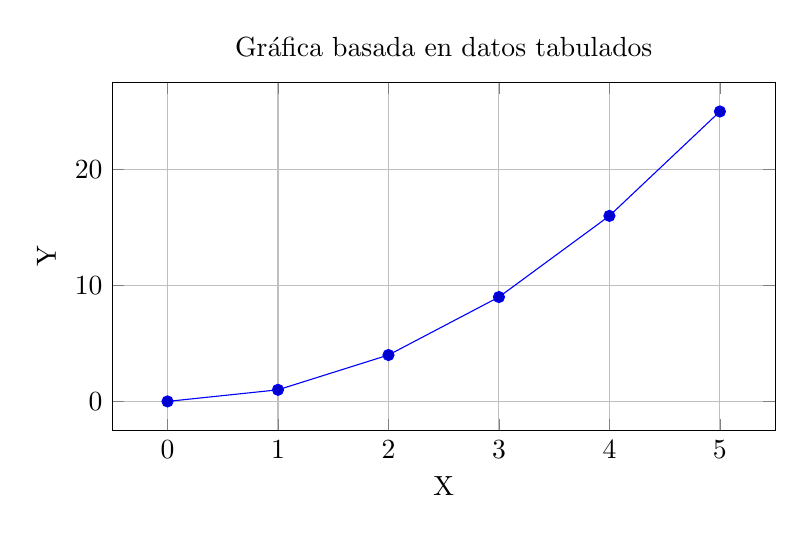
\begin{tikzpicture}
        \begin{axis}[
            title={Gráfica basada en datos tabulados},
            xlabel={X},
            ylabel={Y},
            grid=major, % Añade una cuadrícula mayor
            width=10cm, % Ancho de la gráfica
            height=6cm, % Altura de la gráfica
        ]
        % Datos tabulados para la gráfica
        \addplot table[row sep=\\, y index=1] {
            x y  \\
            0 0  \\
            1 1  \\
            2 4  \\
            3 9  \\
            4 16 \\
            5 25 \\
        };
        \end{axis}
    \end{tikzpicture}
    \caption{Ejemplo de gráfica creada a partir de una tabla de datos}
    \label{fig:tabla_grafica}
\end{figure}
\textbf{\large{\href{https://youtu.be/dQw4w9WgXcQ?si=jGf-LdN459y-xefY}{EJEMPLO DE URL (LINK)}}}
\end{document}